\documentclass[10pt,aspectratio=169]{beamer}

\usetheme[progressbar=frametitle]{metropolis}
\usepackage{appendixnumberbeamer}
%\usecolortheme{orchid}
\usepackage{booktabs}
\usepackage[scale=2]{ccicons}

\usepackage{listings, listings-rust} % To include code listings
\usepackage{xcolor}   % To define custom colors

\usepackage{pgfplots}
\usepgfplotslibrary{dateplot}

% Own images owerlap.
\usepackage{tikz}

% Own QR code
\usepackage{svg}
\usepackage{graphicx}

\usepackage{xspace}
\newcommand{\themename}{\textbf{\textsc{metropolis}}\xspace}

% Own page numbering
\usepackage{lastpage} % To reference the last page number

% Customizing the footline to show Page current page/total pages
\makeatletter
\setbeamertemplate{footline}{
  \begin{beamercolorbox}[wd=\textwidth,ht=3ex,dp=3ex,leftskip=0.3cm,rightskip=0.3cm]{structure}%
  \hfill\usebeamerfont{page number in head/foot}%
    \insertframenumber/\inserttotalframenumber
  \end{beamercolorbox}
}
\makeatother

% Own lst listing.
% Define custom colors for the code listing
\lstdefinestyle{myStyle}{
    belowcaptionskip=1\baselineskip,
    %aboveskip=0pt, % Remove extra space above
    belowskip=0pt, % Remove extra space below
    breaklines=true,
    frame=none,
    numbers=none, 
    basicstyle=\fontsize{7}{9}\selectfont\ttfamily, % Set font size to 7pt
    keywordstyle=\bfseries\color{green!40!black},
    commentstyle=\itshape\color{purple!40!black},
    identifierstyle=\color{blue},
    backgroundcolor=\color{gray!10!white},
}

\title{Why Is Rust the Rising Star?}
%\subtitle{A modern beamer theme}
\author{David Chocholatý}
\institute{Brno University of Technology}
\titlegraphic{\hfill
\includegraphics[height=0.35cm]{img/devconf_logo.png}}
\date{June 14, 2024}

\begin{document}

\maketitle

%\begin{frame}{Table of contents}
%  \setbeamertemplate{section in toc}[sections numbered]
%  \tableofcontents%[hideallsubsections]
%\end{frame}

\section[Why Rust Matters?]{Introduction}

\begin{frame}{Why Rust Matters?}
\begin{columns}
\begin{column}{0.5\textwidth}
    \begin{itemize}
    \setlength\itemsep{1em}
    \item Memory Safe Programming Language
    \pause
    \item Performance Comparable to C and C++
    \pause
    \item Low-Level Control
    \end{itemize}
\end{column}
\begin{column}{0.5\textwidth}  %%<--- here
    \onslide
    \begin{center}
     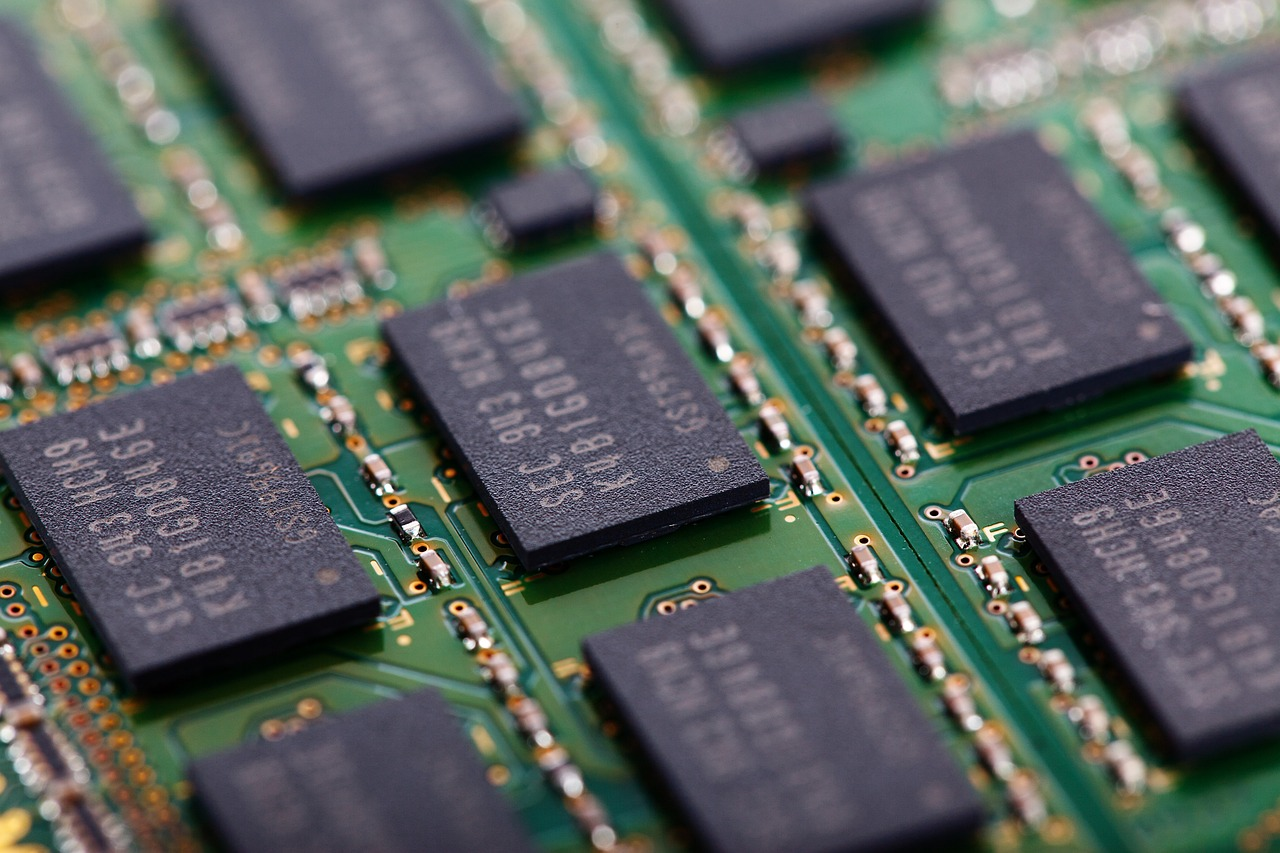
\includegraphics[width=0.675\textwidth]{img/board-22098_1280.jpg}
     \end{center}
\end{column}
\end{columns}
\end{frame}

\begin{frame}{Stay Safe!}
    \begin{center}
        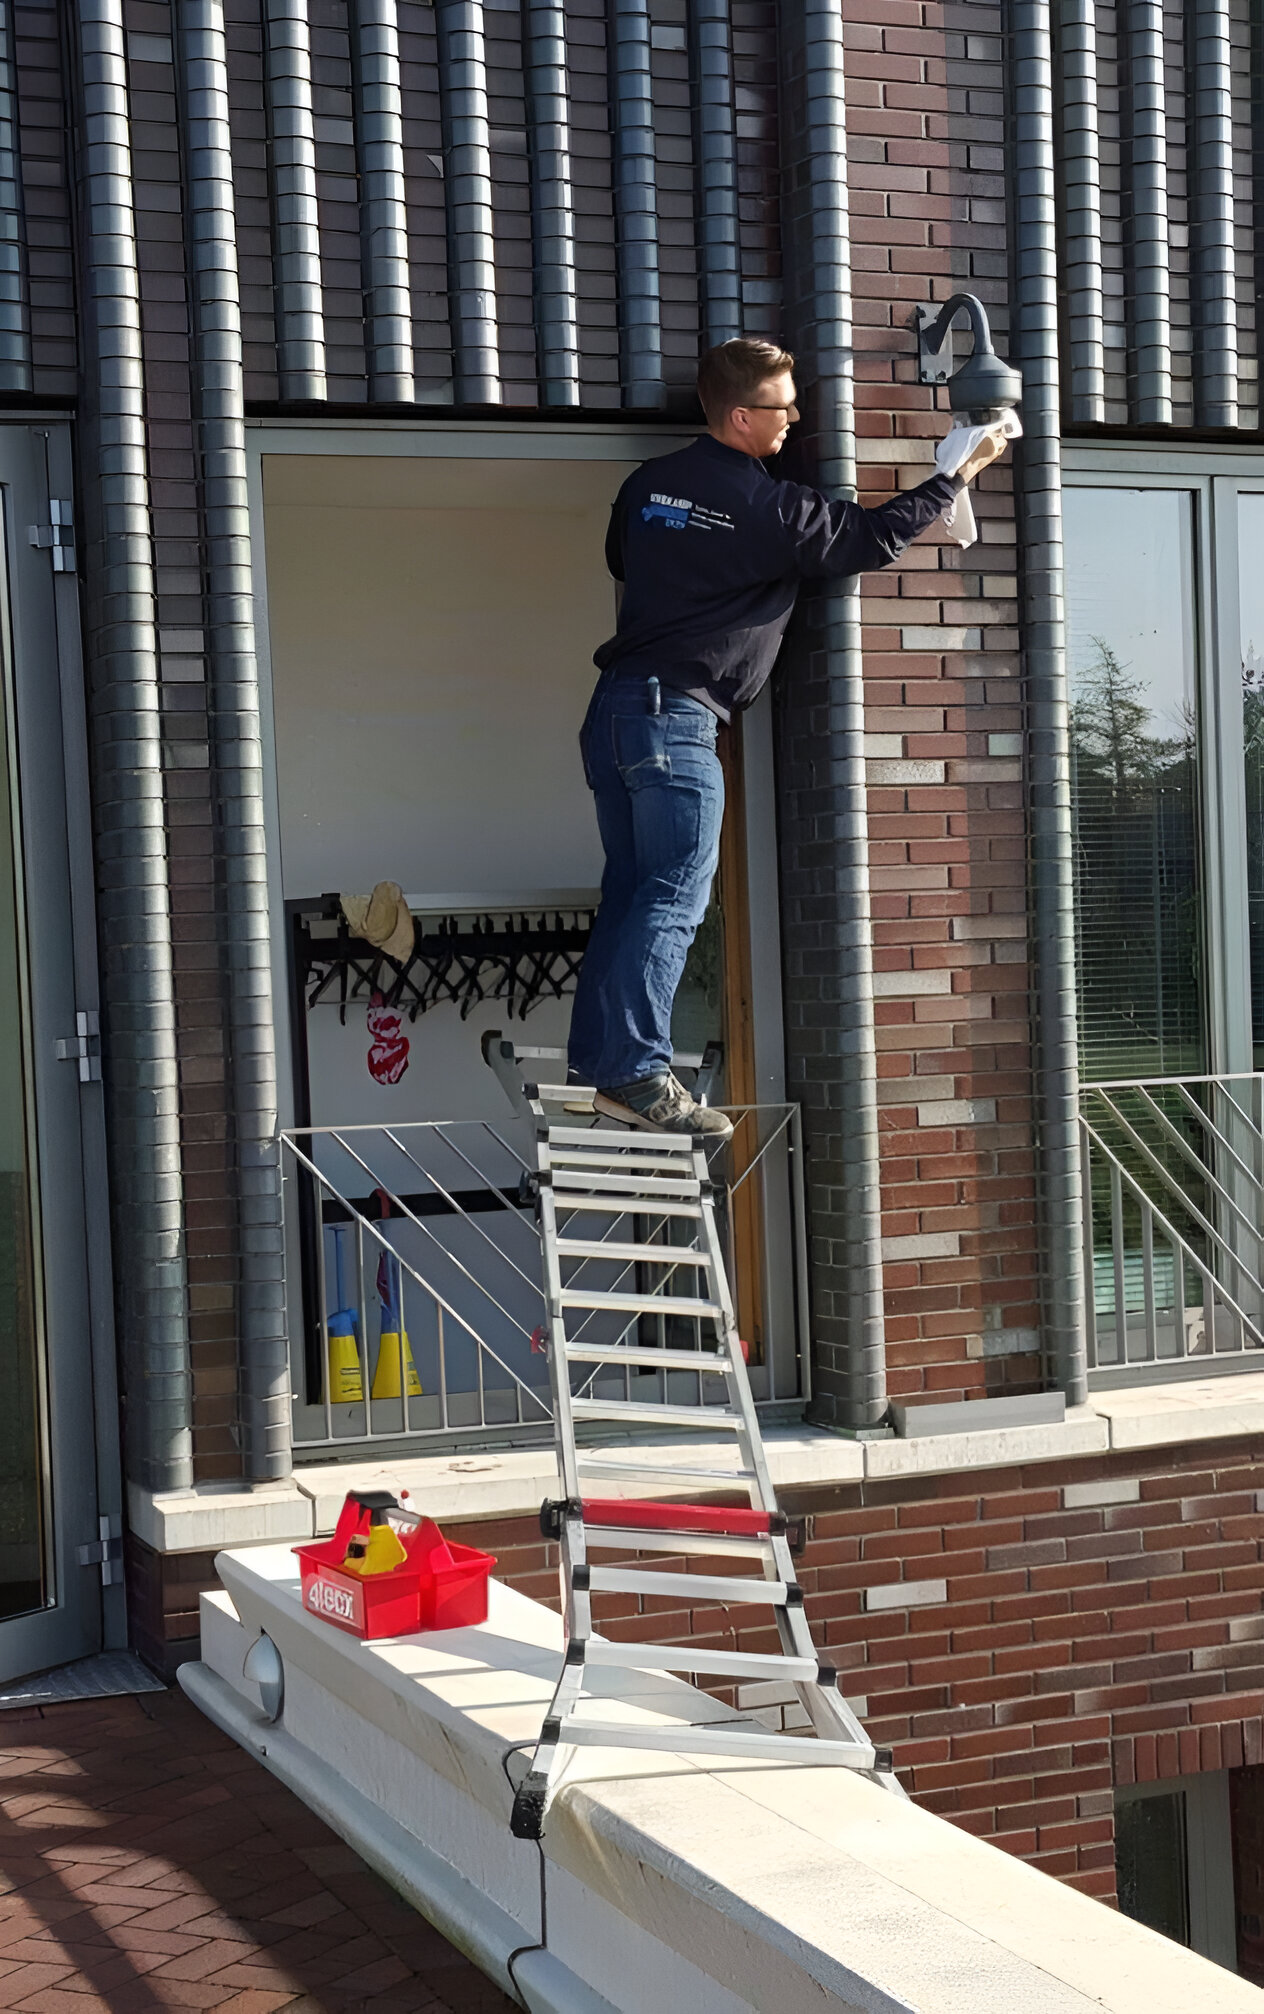
\includegraphics[width=0.34\textwidth]{img/unsafe_work.jpeg}
    \end{center}    
\end{frame}

\begin{frame}{Where Can I Use Rust?}

\begin{columns}
\begin{column}{0.6\textwidth}
    \begin{itemize}
    \item Systems Programming \& CLI Tools
    \item Concurrency and Parallelism
    \item Network Programming
    \item Embedded Systems
    \item Game Development
    \item High-Performance Computing
    \item Blockchain and Cryptography    
\end{itemize}
\end{column}
\begin{column}{0.4\textwidth}  %%<--- here
    \begin{center}
     
\includegraphics[width=0.75\textwidth]{img/mascot.png}
     \end{center}
\end{column}
\end{columns}
\end{frame}

\begin{frame}{Rust in the News}
    \begin{itemize}
        \item \textbf{National Security Agency (USA) urges shift to memory safe programming languages}
        \begin{itemize}
            \item Published: Nov 12, 2022
        \end{itemize}
        \item \textbf{Why Rust is one of the world's most cherished programming languages}
        \begin{itemize}
            \item Published: Feb 26, 2024
        \end{itemize}
        \item \textbf{White House urges developers to dump C and C++}
        \begin{itemize}
            \item Published: Feb 27, 2024
            %\item Source: \url{https://bit.ly/3WYRyoU}
        \end{itemize}
        \item \textbf{Why Rust is emerging as developers’ favourite programming language}
        \begin{itemize}
            \item Published: May 28, 2024
        \end{itemize}
    \end{itemize}    
\end{frame}

\begin{frame}[plain]{We Want the Safety}
    \begin{center}
        \begin{tikzpicture}
            % First image
            \node (img1)  {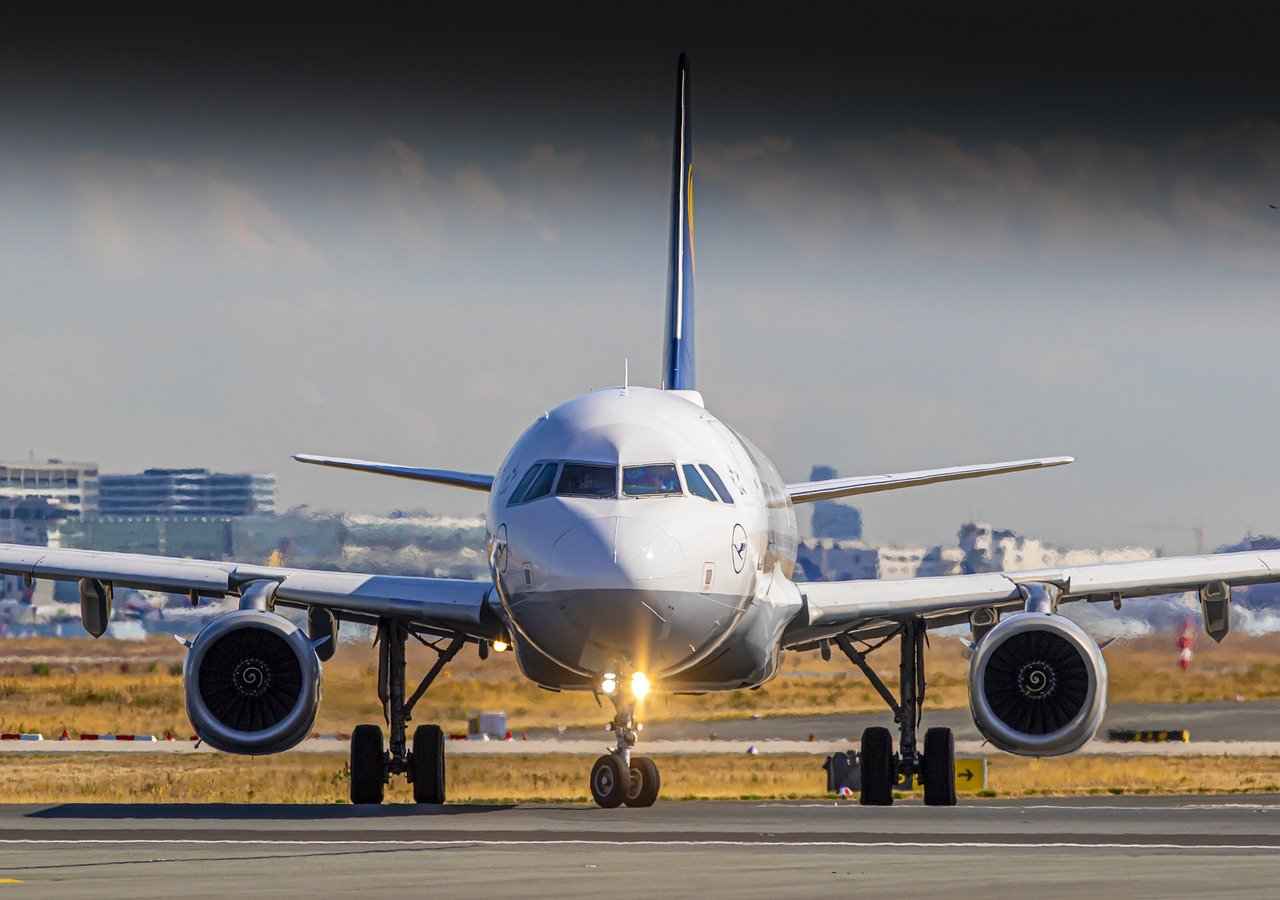
\includegraphics[width=0.45\textwidth]{img/airbus-8607152_1280.jpg}};
            \pause
            % Second image
            \node (img2) at ([xshift=0cm, yshift=0cm]img1.south east) {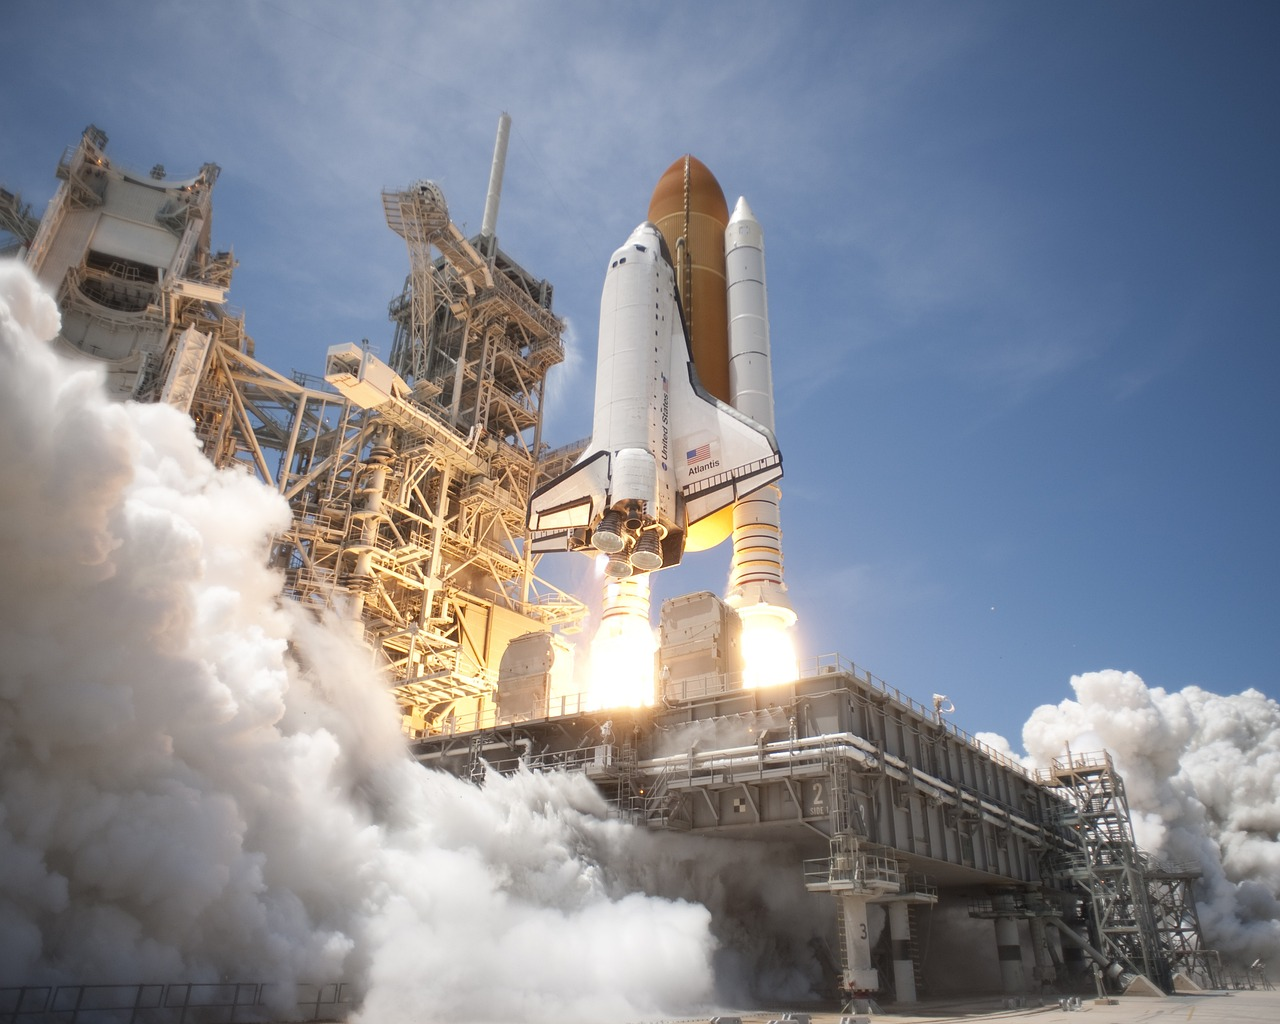
\includegraphics[width=0.45\textwidth]{img/rocket-launch-67721_1280.jpg}};
        \end{tikzpicture}
    \end{center}
    % Overlay page number
% Overlay custom footer with page number
    \begin{tikzpicture}[remember picture,overlay]
        \node[anchor=south west,inner sep=0, xshift=0.992cm, yshift=-1.545ex] at (current page.south west) {
            \begin{beamercolorbox}[wd=\paperwidth,ht=3ex,dp=3ex,leftskip=0.3cm,rightskip=0.3cm]{structure}%
                \hfill\usebeamerfont{page number in head/foot}%
                \insertframenumber/\inserttotalframenumber
            \end{beamercolorbox}
        };
    \end{tikzpicture}
\end{frame}

\section{What Is Rust?}

\begin{frame}{What Is Rust?}
    \begin{itemize}
        \item Safety, Speed, and Concurrency
        \item Developed by Mozilla (Graydon Hoare)
        \item First Stable Release in 2015
        \item Now an Open-Source Project with an Active Community
        \item Extensive Documentation, Tutorials, and Tools
    \end{itemize}
\end{frame}

\begin{frame}{What Is Rust?}

\begin{itemize}
    \setlength\itemsep{4em}
    \item[] {\Large What Do We Mean by \textbf{Safe}?}
    \pause
    \item[]  {\Large Does It Mean That Rust Is \textbf{100\%} Memory Safe?}
    \pause
    \item[] {\Large What Is the Reality of \textbf{Performance}?}
\end{itemize}
\end{frame}

\section{Memory Safety}

\begin{frame}{Memory Safety --- C++ Example}
    \metroset{block=fill}
    % Set custom block background color
    \setbeamercolor{block body}{bg=gray!10!white}
    \begin{block}{C++}        
        \lstinputlisting[
            style=myStyle,
            language=C++
        ]{code/memory_safety.cpp}
    \end{block}
\end{frame}

\begin{frame}{Memory Safety --- Rust Example}
    \metroset{block=fill}
    % Set custom block background color
    \setbeamercolor{block body}{bg=gray!10!white}
    
    \begin{block}{Rust}        
        \lstinputlisting[
            style=myStyle,
            language=Rust
        ]{code/memory_safety.rs}
    \end{block}
\end{frame}

\section{Type System}

\begin{frame}{Type System --- C++ Example}
    \metroset{block=fill}
    % Set custom block background color
    \setbeamercolor{block body}{bg=gray!10!white}
   \begin{block}{C++}        
        \lstinputlisting[
            style=myStyle,
            language=C++
        ]{code/type_system_1.cpp}
    \end{block}
\end{frame}

\begin{frame}{Type System --- C++ Example}
    \metroset{block=fill}
    % Set custom block background color
    \setbeamercolor{block body}{bg=gray!10!white}
    \begin{block}{C++}        
        \lstinputlisting[
            style=myStyle,
            language=C++
        ]{code/type_system_2.cpp}
    \end{block}
\end{frame}

\begin{frame}{Type System --- Rust Example}
    \metroset{block=fill}
    % Set custom block background color
    \setbeamercolor{block body}{bg=gray!10!white}
   \begin{block}{Rust}        
        \lstinputlisting[
            style=myStyle,
            language=Rust
        ]{code/type_system_1.rs}
    \end{block}
\end{frame}

\begin{frame}{Type System --- Rust Example}
    \metroset{block=fill}
    % Set custom block background color
    \setbeamercolor{block body}{bg=gray!10!white}
   \begin{block}{Rust}        
        \lstinputlisting[
            style=myStyle,
            language=Rust
        ]{code/type_system_2.rs}
    \end{block}
\end{frame}

\begin{frame}{Type System --- Rust Example}
    \metroset{block=fill}
    % Set custom block background color
    \setbeamercolor{block body}{bg=gray!10!white}
   \begin{block}{Rust}        
        \lstinputlisting[
            style=myStyle,
            language=Rust
        ]{code/type_system_3.rs}
    \end{block}
\end{frame}

\begin{frame}{Fixed!}
    \begin{center}
        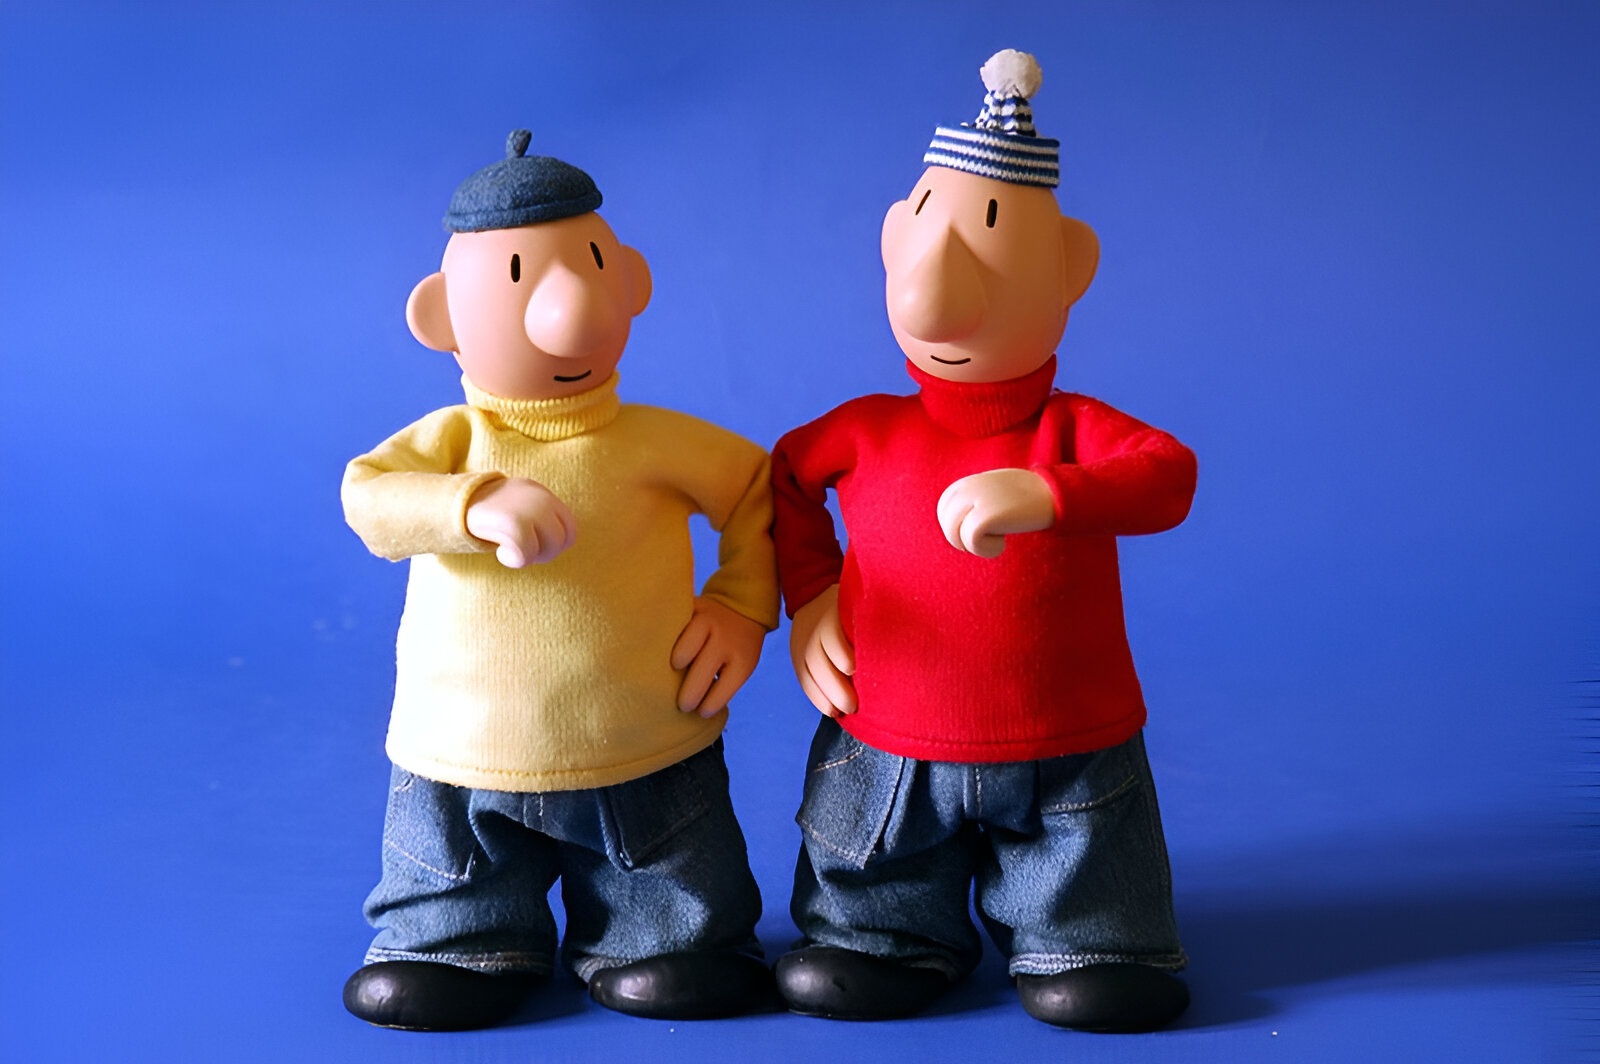
\includegraphics[width=0.75\textwidth]{img/pat_a_mat.jpeg}
    \end{center}    
\end{frame}

\section{Unsafe Rust}

\begin{frame}{Unsafe Rust --- C++ Example}
    \metroset{block=fill}
    % Set custom block background color
    \setbeamercolor{block body}{bg=gray!10!white}
   \begin{block}{C++}        
        \lstinputlisting[
            style=myStyle,
            language=C++
        ]{code/unsafe.cpp}
    \end{block}
\end{frame}

\begin{frame}{Unsafe Rust --- Rust Example}
    \metroset{block=fill}
    % Set custom block background color
    \setbeamercolor{block body}{bg=gray!10!white}
   \begin{block}{Rust}        
        \lstinputlisting[
            style=myStyle,
            language=Rust
        ]{code/unsafe.rs}
    \end{block}
\end{frame}

\section{Performance}

\begin{frame}{Performance}
\begin{itemize}
    \item The Benchmarks Game (\url{https://bit.ly/3X4NLGI})
\end{itemize}

\begin{figure}[htbp]
  \centering
  \resizebox{0.7\textwidth}{!}{%
    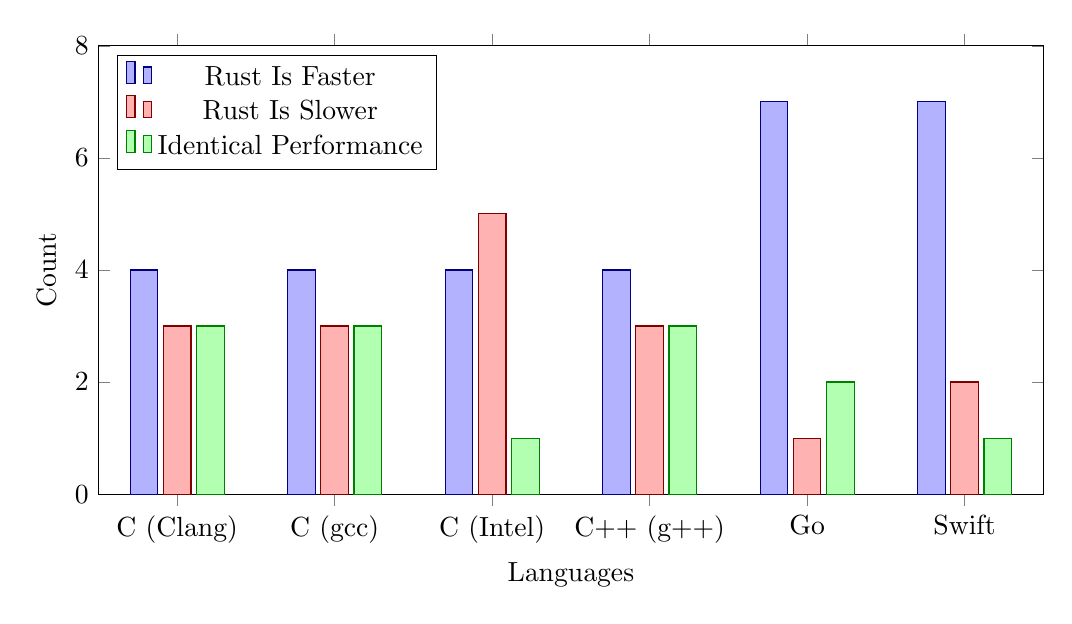
\begin{tikzpicture}
      \begin{axis}[
          ybar,
          ylabel={Count},
          xlabel={Languages},
          symbolic x coords={C (Clang), C (gcc), C (Intel), C++ (g++), Go, Swift},
          xtick=data,
          ymin=0,
          ymax=8,
          legend style={at={(0.02,0.98)},anchor=north west,cells={align=left}},
          cycle list={
            {fill=blue!30!white,draw=blue!50!black},
            {fill=red!30!white,draw=red!50!black},
            {fill=green!30!white,draw=green!50!black}
          },
          bar width=10pt, % Adjust the width of the bars
          x=2cm, % Increase the distance between the groups
      ]
      \addplot coordinates {(C (Clang), 4) (C (gcc), 4) (C (Intel), 4) (C++ (g++), 4) (Go, 7) (Swift, 7)};
      \addplot coordinates {(C (Clang), 3) (C (gcc), 3) (C (Intel), 5) (C++ (g++), 3) (Go, 1) (Swift, 2)};
      \addplot coordinates {(C (Clang), 3) (C (gcc), 3) (C (Intel), 1) (C++ (g++), 3) (Go, 2) (Swift, 1)};
      \legend{Rust Is Faster, Rust Is Slower, Identical Performance}
      \end{axis}
    \end{tikzpicture}%
  }
  \caption{Comparison of Rust Performance with Other Languages}
\end{figure}
\end{frame}

% Done
% Memory Safety (Highlight Rust's unique ownership system, which ensures memory safety without a garbage collector.)
% Type System: Rust has a strong, static type system that catches many errors at compile time, ensuring greater reliability and correctness in programs.
% Error handling
% Concurrency (Discuss Rust's concurrency model, which helps prevent data races and makes writing concurrent code easier and safer.)
% Performance (comparision with C and C++)
% Zero-Cost Abstractions: Rust offers high-level abstractions without compromising performance. These abstractions are compiled away, so there's no runtime overhead.
% Package management - Cargo package manager and other tools (Tooling: Rust comes with excellent tooling, including Cargo (its package manager and build system), rustfmt (for automatic code formatting), and Clippy (a linter to catch common mistakes).)
% Unsafe Rust
% Zminit uzitecne linky (Crates.io, dokumentaci, ...)

\begin{frame}{Presentation Hosted on GitHub}
    \begin{itemize}
        \item The Presentation and Source Codes Available on:
    \end{itemize}

    \begin{center}
        \url{https://bit.ly/3KsMh1y}    
    \end{center}    

    \begin{center}
        
\includegraphics[width=0.375\textwidth]{img/qr.pdf}
    \end{center}
\end{frame}

\begin{frame}{Coding in Rust Is Hard ...}
    \begin{center}
        
\includegraphics[width=0.75\textwidth]{img/minion.jpeg}
    \end{center}
\end{frame}

\begin{frame}{But It Makes Sense!}
\begin{center}
    
\includegraphics[width=0.75\textwidth]{img/meme.png}
\end{center}
\end{frame}

\section{Why Is Rust the Rising Star?}

{\setbeamercolor{palette primary}{fg=black, bg=yellow}
\begin{frame}[standout]
  Questions?
\end{frame}
}

\appendix

\begin{frame}[allowframebreaks]{References}
    \invisible<1->{\cite{infoworld2024whitehouse,dod2022software,linkedin2023memorysafety,memorysafety2024,nsa2023,threatdown2024,benchmarksgame2024,thenextweb2024,thirdact2024,cratesio,rustlangbook,rustbyexample,rustlings,awesomerust,wikimedia2024rustmascot,airbus,pixabay2024rocket,skoolcool2017,ahmadturk2014,pixabay22098,bairesdev2024,pat_mat_2014,unsafe_work}}
  \bibliography{demo}
  \bibliographystyle{abbrv}

\end{frame}

\end{document}
